\begin{figure}[H]
  \begin{center}
    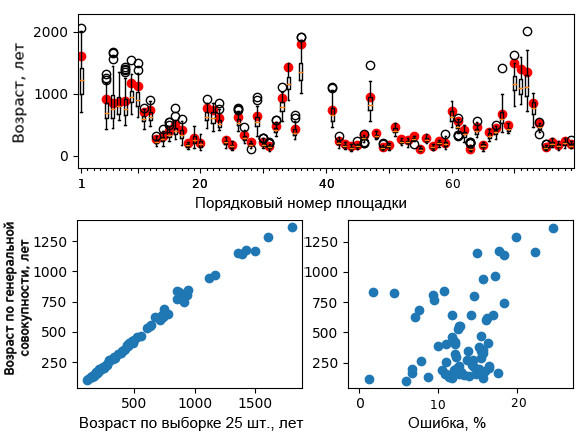
\includegraphics[width=0.95\textwidth]{authors/kolegov-fig2.jpg}
  \end{center}
  \vspace{-0.5cm}
  \caption{График распределения выборок (\textit{а}). Красными точками показаны истинные значения,
полученные по 100 замерам, чёрные боксы и кружки~--- выборки из 25 шт. Графики ошибок: \textit{б}~--- график зависимости истинных значений от выборки в 25 ед.; \textit{в}~--- погрешность измерений, получаемая при замере 25 талломов}
  \label{fig:kolegov}
\end{figure}
